\section{Results}\label{sec:results}

References beginning with S1, S2, or S3 point to the Supplementary Material (one separate file). AUCs are in percent and differences in percentage points (pp).

\subsection{Cohort characteristics and study population}\label{sec:populasi}

Epilepsy labels and acquisition conditions were associated in this cohort: the epilepsy group was younger (median 52 vs 59 years) and was recorded in different eras and on different devices (\tabref{tab:kohort}).
Of 265 first-session recordings in TUEP v2.0.1, 249 recordings (78.3 hours) were analyzed and yielded 26,968 clean 10 s windows from 200 patients (12--411 per patient), with no patients excluded; 100 patients had epilepsy and 100 did not. \figref{fig:sinyal} gives an example of the signal.
The median age was 55 years (range 13--88); sex, montage, sampling frequency, and recording duration did not differ between the groups ($p = 0.13$--$0.57$).
Patients with epilepsy had more clean windows and more sessions in the corpus (\tabref{tab:kohort}); later sessions were not used for training or for the main evaluation.
Year and device are inputs of the metadata baseline (year $\leq$2009: 25 vs 6; Alliance: 12 vs 1), so this baseline reached an AUC of 65.5 and fell to 43.2 when both were matched (Subsection~\ref{sec:strata}).

\begin{table}[t]
\caption{Characteristics of TUEP patients at the first session. The $p$ values use the Mann--Whitney test (age, duration, windows, sessions), Fisher's test (sex), and the chi-squared test (era, device, montage, sampling frequency). IQR is the interquartile range; the average reference includes one patient with the AR(A) variant.}\label{tab:kohort}
\centering\scriptsize
\setlength{\tabcolsep}{2.5pt}
\begin{tabular}{p{0.34\textwidth}cccc}
\toprule
Characteristic & All & Epilepsy & Non-epilepsy & $p$ \\
\midrule
Patients, $n$ & 200 & 100 & 100 & \\
Age, median [IQR] (years) & 55 [45--69] & 52 [43--63] & 59 [47.8--76] & 0.002 \\
Female, $n$ (\%) & 109 (54.5) & 59 (59.0) & 50 (50.0) & 0.256 \\
Era $\leq$2009 / 2010 / 2011 / 2012 / 2013, $n$ & 31/32/42/48/47 & 25/16/20/24/15 & 6/16/22/24/32 & 0.0013 \\
Device X / Intuition / Alliance / other, $n$ & 140/38/13/9 & 65/17/12/6 & 75/21/1/3 & 0.0096 \\
Duration of first-session recording, median [IQR] (minutes) & 21.1 [20.2--23.2] & 21.3 [20.2--24.1] & 20.9 [20.1--22.8] & 0.13 \\
Clean windows per patient, median [IQR] & 123 [117--134] & 124 [118--141.2] & 122 [116--132.2] & 0.027 \\
Sessions per patient in the corpus, median [IQR] & 2 [1--3.2] & 3 [2--6.2] & 1 [1--2] & $9.9\times10^{-13}$ \\
\bottomrule
\end{tabular}
\end{table}

\subsection{Properties of the audit rules}\label{sec:oc}

When leakage was absent, the absolute rule almost never declared leakage. The paired rule did so mainly for raw tree pipelines in the plasmode. Both rules often withheld the decision ``no evidence'' when there were few replicates or a large replicate spread (\tabref{tab:oc}).
With 20 replicates, the unadjusted pipelines on real EEG features in scenario H1 received the R1 decision ``leakage'' in 0.0\% of draws and ``no evidence'' in 92.8\%--100\%; across 396 simulation cells without leakage the mean frequencies were 0.1\% (maximum 7.0\%) and 91.3\%.
Leakage of known size was detected: the control-referenced adjustment (mean null AUC 56.0) was classified as leakage in 87.8\% of draws of 20 replicates (Monte Carlo 95\% CI 61.3\%--98.3\%) and 99.6\% of draws of 100, and simulation cells with a long-run AUC above 55 in 95.9\%. Between 52 and 55 the decision was usually ``uncertain'', as the rule intends.
The paired rule behaved alike in the simulation (no leakage: ``leakage'' in 0.4\%; leakage above 3 pp: 96.2\%), but on raw features with tree classifiers in the plasmode at $\gamma=0$, where no leakage is possible, the stored replicates had mean differences of +2.2 to +3.0 pp with an SD of 7.2--7.8 pp, and ``leakage'' was declared in 31.5\%--48.0\% of draws of 20 replicates. Under a normal model with a true difference of zero and an SD of 7.8 pp, the false-alarm frequency is 4.2\% with 20 replicates and falls below 1\% only with 50 replicates, whereas ``no evidence'' is reached in only 53.4\% and 81.4\% (S2.15). Extending these four pools to 120 replicates (round 50) shrank their mean differences to +0.9 to +1.1 pp (95\% CIs including zero; SD 7.5--8.0 pp) and the frequency of ``leakage'' to 10.7\%--13.9\% with 20 replicates, 2.7\%--4.2\% with 50, and 0.3\%--0.8\% with 100, whereas ``no evidence'' stayed at 45.6\%--52.1\% with 50 or 100 replicates because the pool means lie at the 1.0 pp threshold (S2.16).
The SE in the rules described Monte Carlo error adequately: the patient-bootstrap SD of the mean null AUC of C1 over 100 replicates (0.34 pp) did not exceed its Monte Carlo SE (0.43 pp) (conjecture: every replicate draws a new permutation, and its spread already contains the sampling noise of an AUC on 200 patients).
Under thresholds that were stricter or looser by 1 pp, the decisions ``leakage'' for raw adjustment (V0, \textit{random forest}, XGBoost, Bi-LSTM) did not change, whereas the decisions about the mitigations were threshold-dependent: rank-normal with a \textit{random forest} moved from ``no evidence'' to ``uncertain'' under the stricter set, rank-normal with XGBoost from ``uncertain'' to ``no evidence'' under the looser set, and rank-normal with the Bi-LSTM from ``leakage'' to ``uncertain'' (R1) under the looser set (2 of 18 R1 and 1 of 5 R2 decisions on the real EEG pools changed per set).

\input{\naskahdir/tabel_oc}

\subsection{Adjustment failure in the originally planned pipeline}\label{sec:kebocoran}

The covariate adjustment fitted from training controls only (V0; Subsection~\ref{sec:model}) leaked covariates into features without disease information, consistent with its fitting patients being selected by label; adjustment fitted on all training patients (V4) showed no evidence of leakage in this test.
In the test with uninformative features of the Hamdan et al. type \cite{hamdan2023} (50 canonical folds; \tabref{tab:kebocoran_badan}; \tabref{tab:hamdan}), C1 gave a pooled AUC close to chance (50.8; 5th--95th percentile: 45.1--56.8 for H1). In the planned audit (round 28), I2 based on V0 without age and sex reached 56.4 (51.1--62.4) for H1 and 55.8 for H2a, above the threshold of 55 set beforehand.
A separate reference from half of the training controls (V1) and a \textit{cross-fitted} scheme (V2) did not remove the leakage, and their scores still depended on era ($p_{\mathrm{Holm}} \leq 0.003$; \tabref{tab:sensitivitas}). With V4 the score fell to 50.4 for H1 and 51.7 for H2a, and no dependence on era was found ($p = 0.98$). On the per-fold AUC, the R1 decision was the same for all six variants (V0 56.9; V4 50.0; \tabref{tab:s2_p46}).
For P3 the earlier adjustment leaked (55.5) and V5 showed no evidence of leakage (49.8 and 50.0), and for NM V4 lowered 56.1 to 51.5 (20 replicates; \tabref{tab:kebocoran}).
F2 with V0 originally reached 73.5 per fold (95\% CI 65.6--81.3) and 69.7 (61.0--78.5) after the leaking adjustment was replaced.
That decrease ($-3.7$ pp; $p = 0.14$; lower in 39 of 50 folds) cannot yet be distinguished from variation between folds.

\input{\naskahdir/tabel_kebocoran_badan}

\subsection{Leakage map: simulation, within-patient structure, and plasmode}\label{sec:peta}

Leakage by adjustment depended on the shape of the feature distribution and on the classifier type, not on adjustment alone.
In the simulation without a disease signal (\tabref{tab:peta_sim}; \figref{fig:peta}), per-patient adjustment raised the AUC of nonlinear classifiers when the features were heavy-tailed. The mean per-fold difference was +6.5 pp for raw features (60.0\% of cells with the decision ``leakage''), +3.9 pp for symlog with $c=1$ (37.1\%), +0.2 pp for log (lognormal data), and $-$0.1 pp for rank-normal (0\% ``leakage'').
Logistic regression did not show this pattern (134 cells; maximum difference +2.6 pp).
Recomputation on the per-fold AUC changed the decision category in 7 of 430 cells for R1 and 6 of 366 cells for R2 (1.6\% each), all in the ``uncertain'' category. The conjectures that the pooled AUC pushes the baseline below 50 (H40-1) and that skewness, residual quantiles, or the symlog kink explain the difference better than kurtosis (H40-3) were not supported (out-of-sample $R^2$ $-$0.270 and $-$21.688). No tail property that explains the leakage has therefore been identified; the map is reported empirically, not as a theory.
To isolate the within-patient structure, the simulation kept the number of patients, the marginal feature distribution, and the covariates fixed and varied the intraclass correlation (ICC) of the windows, the number of windows, and the order of aggregation (Subsection~\ref{sec:metode_peta}; \figref{fig:struktur}; \tabref{tab:s2_struktur}).
With heavy-tailed features, adjustment before window-level classification raised the AUC of the \textit{random forest} in all 24 cells (mean +3.9 to +14.6 pp; 95\% CI above zero in every cell), whereas with normal features no cell differed from zero (largest absolute mean 1.4 pp).
The leak was not shown to grow with the correlation of the windows: in the primary family, the change from latent ICC 0 to 0.95 (lognormal, 50 windows) was $-$1.8 pp (95\% CI $-$6.3 to +2.7; Holm 0.79), and the mean at ICC 0.95 was below the mean at ICC 0 in all six combinations of heavy-tailed distribution and number of windows.
Aggregating to patient means before adjusting left a leak of only +0.5 to +0.9 pp at ICC 0 with lognormal features and was better than window-level adjustment by +8.9 pp in one simulated cell (lognormal, 50 windows, ICC 0; 95\% CI +6.0 to +11.8; Holm $<0.001$), but this advantage shrank to +0.1 pp at ICC 0.95 (lognormal, 50 windows), where the aggregated arm itself leaked +7.6 pp. Descriptively and without a test, the same contrast with lognormal features was +10.2, +8.9, and +10.1 pp at ICC 0 and +1.6, +0.1, and +0.6 pp at ICC 0.95 for 10, 50, and 200 windows.
With 1\% contaminated features and 10 windows per patient, aggregation did not avoid the leak even at ICC 0 (+11.8 pp), and patient-level logistic regression stayed within 3.3 pp of zero in every cell.
Here the number of windows per patient was constant, so adjustment per window and per patient gave identical results; with unequal counts (12--200 windows per patient; round 39), the two adjustments differed by at most 0.8 pp in pooled AUC across ten classifier--distribution cells.

\begin{figure}[t]
\centering
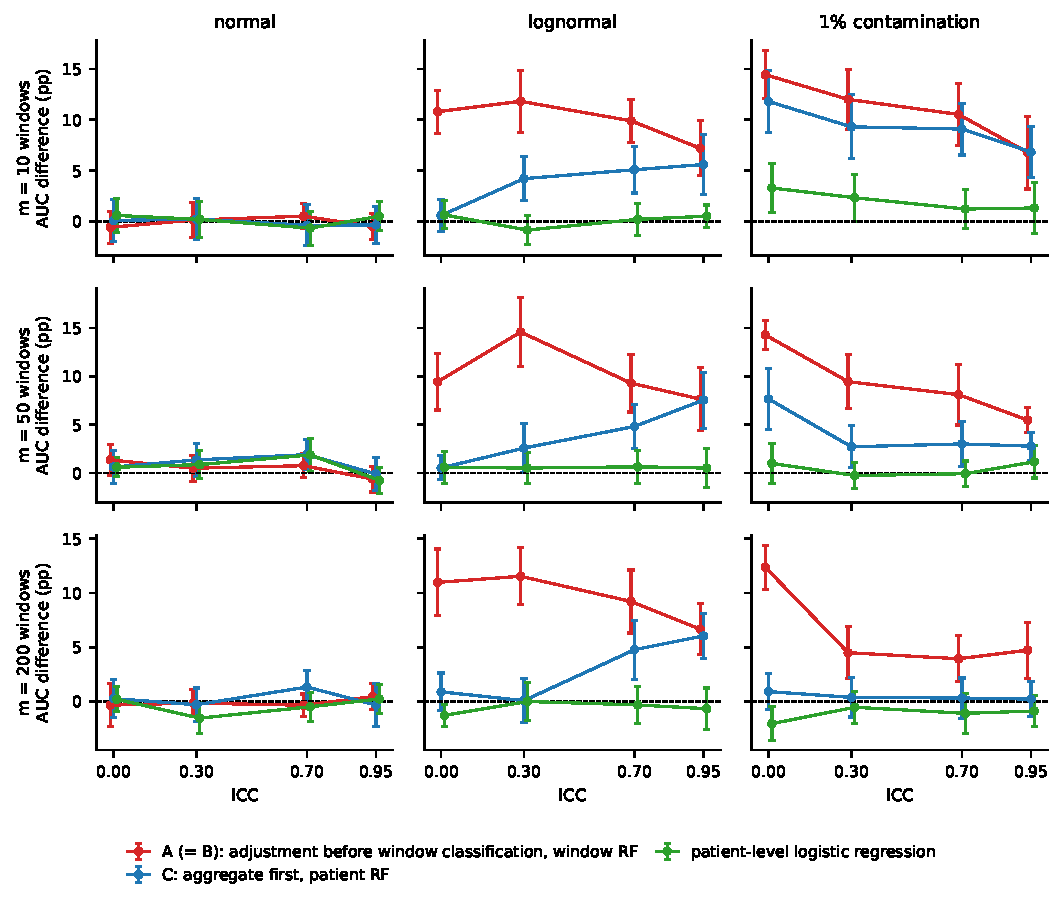
\includegraphics[width=0.95\textwidth]{figures_en/hasil_struktur49.pdf}
\caption{Within-patient structure in simulated data without a disease signal ($n=200$ patients, 20 features, 20 replicates per cell). AUC difference in pp (with minus without adjustment; points: mean, bars: $\pm$1.96 SE) by the latent intraclass correlation (ICC) of the windows, for three marginal distributions (columns) and 10, 50, and 200 windows per patient (rows). A: adjustment before window-level classification (window-level \textit{random forest}); C: aggregation to patient means before adjustment (patient-level \textit{random forest}); LR: patient-level logistic regression. Arm B (adjustment from patient means applied to windows) coincides with A because the number of windows per patient was constant. Dashed line: zero.}\label{fig:struktur}
\end{figure}

\begin{figure}[t]
\centering
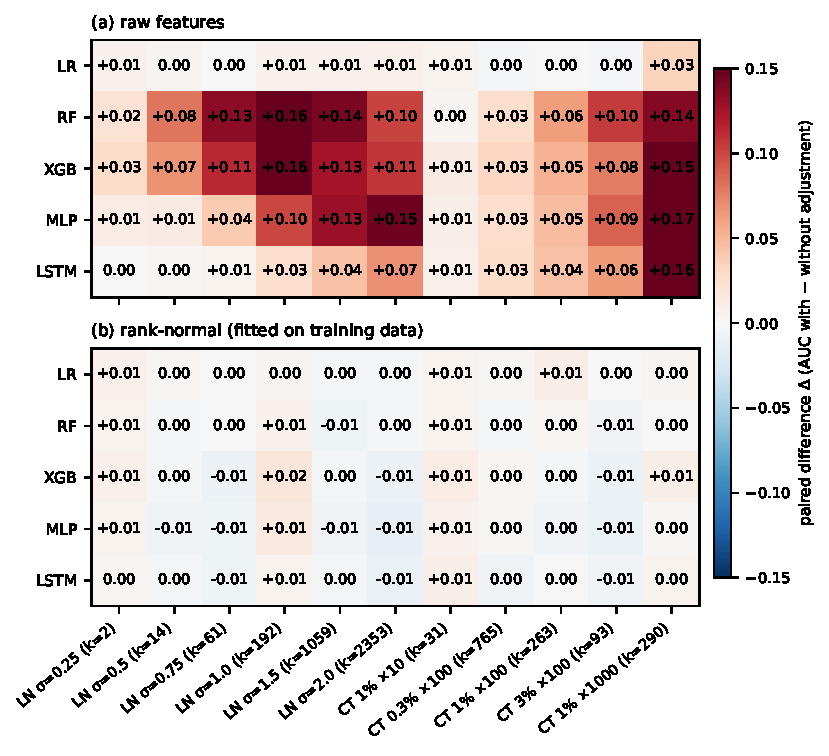
\includegraphics[width=0.72\textwidth]{figures_en/hasil_peta_kebocoran.pdf}
\caption{Covariate leakage map on simulated data without a disease signal (H1 scenario, $n=200$ patients, 50 windows, 50 features). The panels show the paired difference in AUC (with minus without patient-level covariate adjustment) for five classifiers (LR: per-patient logistic regression; RF: \textit{random forest}; XGB: XGBoost; MLP; LSTM: Bi-LSTM) on: (a) raw features and (b) rank-normal fitted on the training data. The horizontal axis contains the lognormal distribution (LN with deviation parameter $\sigma$) and contamination (CT with sample percentage $f$ and deviation multiplier scale $c$); $k$ is the mean empirical kurtosis. The symlog and log transformations are reported in the text and Table~\ref{tab:peta_sim}.}\label{fig:peta}
\end{figure}

With synthetic labels derived from covariates alone, raw adjustment made three nonlinear classifiers appear informative, and rank-normal reduced this for two of them (\tabref{tab:plasmode}; \figref{fig:plasmode}).
In the plasmode, real EEG features were swapped between patients and synthetic labels were generated from covariates alone ($\gamma=1$ mimics the real association; covariate AUC 70.7 versus 71.0).
Per-patient adjustment of raw features leaked into the \textit{random forest} (per-fold AUC 60.9 versus 50.4 without adjustment), XGBoost (62.4 and 50.5), and the Tang Bi-LSTM (63.6 and 51.7), increasing with $\gamma$.
Rank-normal reduced this to 51.3 for the \textit{random forest} and 51.1 for XGBoost (difference from the raw pipeline +9.6 and +11.3 pp; Holm $<0.001$), but only to 55.6 for the Bi-LSTM (R1 ``leakage''; difference +8.0 pp).
For NM (20 replicates), the per-fold AUC at $\gamma=1$ was 50.5 without covariate regression, 50.9 with V4, and 50.3 with rank-normal before V4 (R2 ``no evidence'' for both). The null test with real labels over 50 replicates gave a difference of +1.9 pp ($p = 0.003$; per-fold R1 ``uncertain''), so NM-V4 did not fully pass.
The control at $\gamma=0$ was met for logistic regression, the \textit{random forest}, and Tang but not for XGBoost (7 of 10 cells); this failure limits the conclusions for XGBoost to the leakage at $\gamma=1$, which was large (+11.9 pp). The \textit{random forest} with IPW showed no evidence of leakage (6 of 6 cells; AUC 50.2 at $\gamma=1$ versus 60.9 for raw adjustment).
Rank-normal reduced leakage in both tree-based classifiers, but not completely in the Bi-LSTM, and its ``no evidence'' decisions depended on the thresholds (Subsection~\ref{sec:oc}).
In the independent Emotiv cohort (round 50; \tabref{tab:plasmode}), raw per-patient adjustment again leaked into the \textit{random forest} (per-fold AUC 61.6 versus 48.8 without adjustment; +12.7 pp, 95\% CI +10.4 to +15.0) and XGBoost (60.5 versus 48.9; +11.6 pp, +9.0 to +14.2; Holm $<0.001$ for both), whereas logistic regression stayed within 0.3 pp of its unadjusted pipeline in every cell. Rank-normal lowered the leak by 11.3 and 10.5 pp but left +1.4 and +1.0 pp (R2 ``uncertain''), and all 12 adjusted cells at $\gamma=0$ passed the control.

\begin{figure}[t]
\centering
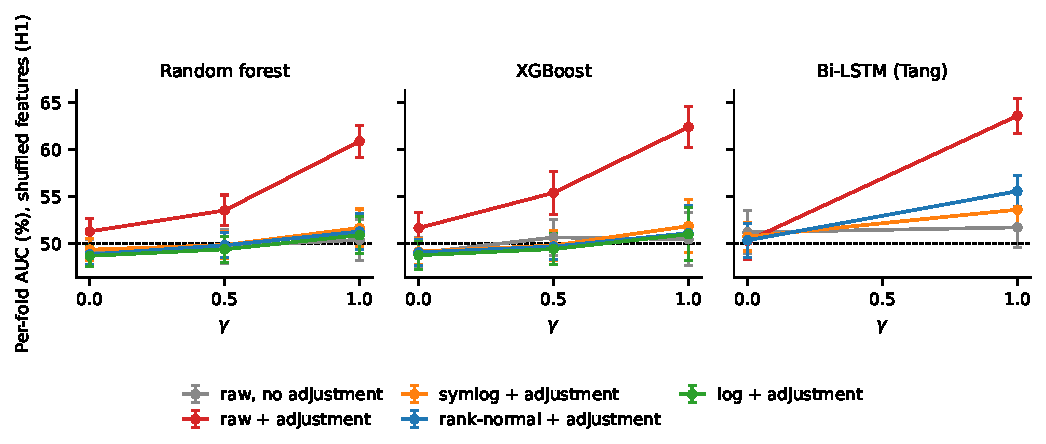
\includegraphics[width=0.78\textwidth]{figures_en/hasil_plasmode.pdf}
\caption{Plasmode results on real TUEP EEG features with labels synthesized purely from covariates (condition H1). Mean per-fold AUC by covariate interaction parameter $\gamma \in \{0, 0.5, 1\}$ for the \textit{random forest}, XGBoost, and the Tang Bi-LSTM under various feature transformations.}\label{fig:plasmode}
\end{figure}

\input{\naskahdir/tabel_plasmode}

\subsection{Implications for classification of the TUEP label}\label{sec:kinerja}

The acquisition-metadata baseline without EEG reached a per-fold AUC of 65.5, close to the F2 score, so a good-looking EEG score cannot yet be separated from acquisition information (\tabref{tab:utama}; \figref{fig:kinerja}).
F2 reached a per-fold AUC of 69.7 (Nadeau--Bengio corrected 95\% CI 61.0--78.5; SD 8.4) and a pooled AUC of 69.4; these outputs combine EEG with age and sex.
Combined with all non-EEG predictors, the EEG features added +7.6 pp (N1 73.8 versus N0 66.1; 95\% CI $-$1.0 to +16.2; $p = 0.082$) and the unadjusted band powers +8.2 pp (N2 74.3; $p = 0.071$; Holm 0.14 for both), so additional information in the EEG beyond these predictors was not established by the corrected test (patient bootstrap with fixed models: CIs +0.1 to +13.2 and +0.2 to +13.7 pp).
Refitting every transform inside the inner folds changed the per-fold AUC by at most 0.3 pp for every model, including NM and F2 (F2 +0.3 pp; 95\% CI $-$3.5 to +4.2), even though the NM configuration $(d, L)$ chosen differed from the original in 27 of 50 folds, and the strict F2 still did not differ significantly from the strict metadata baseline or C1 (S2.15).
The demographic baseline reached 62.0; sensitivity, specificity, and BAC at the 0.5 threshold are descriptive and were not used for inference.

\begin{table}[t]
\caption{Performance of from-scratch models with covariate adjustment and non-EEG baselines under the patient-level protocol with 50 canonical folds. AUC in percent; the 95\% CI of the per-fold AUC is Nadeau--Bengio corrected and the CI of the pooled AUC uses patient-level \textit{bootstrap}; metrics at the 0.5 threshold are descriptive and averaged over 10 repetitions. I2, P3, NM, F2, and C1 include age and sex. N0--N2 use strict nesting (round 49). Sens is sensitivity, Spec specificity, BAC balanced accuracy, and NA not available.}\label{tab:utama}
\centering\scriptsize
\setlength{\tabcolsep}{3pt}
\begin{tabular}{p{0.40\textwidth}ccccc}
\toprule
Model & Per-fold AUC [CI] & Pooled AUC [CI] & Sens & Spec & BAC \\
\midrule
\textbf{F2 (I2 + P3 + NM)} & 69.7 [61.0--78.5] & 69.4 [63.3--75.5] & 65.0 & 63.0 & 64.0 \\
I2 & 68.0 [59.2--76.9] & 67.8 [61.1--74.2] & 66.7 & 62.2 & 64.5 \\
P3 & 66.6 [58.5--74.6] & 65.3 [58.9--71.3] & 60.9 & 62.8 & 61.9 \\
NM & 67.0 [58.8--75.2] & 66.3 [60.3--72.1] & 63.3 & 59.8 & 61.6 \\
C1 (no covariate adjustment) & 67.5 [59.0--76.0] & 66.6 [60.3--73.2] & 64.9 & 60.2 & 62.6 \\
\midrule
Acquisition-metadata baseline (no EEG) & 65.5 [56.5--74.5] & 64.8 [57.7--70.9] & 44.8 & 73.5 & 59.2 \\
Demographic baseline (age + sex) & 62.0 [52.3--71.6] & 60.0 & NA & NA & NA \\
N0: metadata + age + sex (no EEG) & 66.1 [56.5--75.7] & 66.6 [60.1--73.0] & 54.3 & 67.1 & 60.7 \\
N1: N0 + adjusted I2 features & 73.8 [66.0--81.5] & 73.3 [66.8--79.5] & 68.6 & 67.1 & 67.8 \\
N2: N0 + unadjusted band powers & 74.3 [66.4--82.2] & 73.6 [67.1--80.0] & 68.4 & 68.5 & 68.5 \\
\bottomrule
\end{tabular}
\end{table}

\begin{figure}[t]
\centering
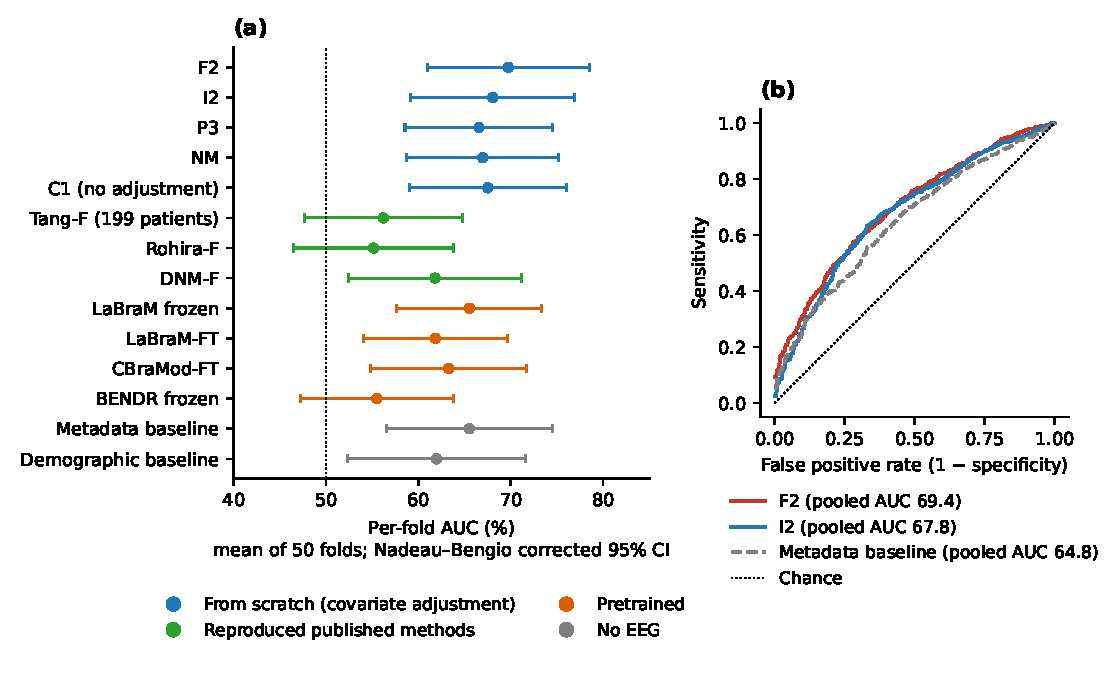
\includegraphics[width=0.80\textwidth]{figures_en/hasil_kinerja.pdf}
\caption{Performance on the 50 canonical folds (TUEP, 200 patients, first session). (a) Per-fold AUC (mean of 50 folds) with Nadeau--Bengio corrected 95\% CI for from-scratch models with covariate adjustment (C1 without adjustment), reproduced published methods without adjustment (Tang-F on 199 patients), \textit{pretrained} comparators, and non-EEG baselines; dashed lines mark an AUC of 50. (b) Mean ROC curve over 10 repetitions for F2, I2, and the metadata baseline; the numbers in the legend are pooled AUCs.}\label{fig:kinerja}
\end{figure}

Fusing three views and adjusting for covariates were not shown to raise the AUC, and F2 was not shown to exceed the metadata baseline ($p = 0.45$--$0.84$ for the four differences; \tabref{tab:uji}). In the post hoc analysis, none of the 12 model pairs was shown to be equivalent at a margin of 3 pp (Holm 1.00; the same at a margin of 2 pp). The smallest SE (2.4 pp) exceeds the 1.8 pp required at that margin, so the test could not pass with 200 patients. At a margin of 5 pp, F2 without NM versus C1 and I2 versus C1 met the TOST criterion before correction ($p = 0.037$) but not after Holm (0.45). The combined effect of covariate adjustment was +2.1 pp ($p = 0.39$; \figref{fig:penyesuaian}a).
I2 was higher than Tang-F and Rohira-F, and F2 was higher than Rohira-F ($q = 0.069$ for all three, not passing FDR 0.05; \tabref{tab:uji}); I2 did not differ significantly from DNM-F (+6.2 pp; $p = 0.31$).
Against the fine-tuned foundation models, F2 was not shown to exceed LaBraM-FT or CBraMod-FT (Holm 0.179 for both; \tabref{tab:uji}). In the patient-level bootstrap (\tabref{tab:s2_p45b}), the differences of F2 against I2, C1, and the metadata baseline remained indistinguishable, but against CBraMod-FT it differed significantly (+6.8 pp; 95\% CI 1.6--11.5; Holm 0.032).
The difference against CBraMod-FT appeared only in the \textit{bootstrap}, which treats the model as fixed and gives narrower CIs than the corrected test (S2).
Predictions from TUEP were not shown to transfer to the two other public cohorts (\tabref{tab:transfer}; S3): I2 with adjustment was lower than C1 on Kural et al. (difference $-5.1$ pp; $p = 0.028$), and the \textit{band-power} model reached 56.5 on Emotiv with frozen TUEP statistics and 54.1 after standardizing each cohort with its own unlabeled features. These transfer analyses test predictions, not the audit protocol.
\input{\naskahdir/tabel_transfer}

\begin{table}[t]
\caption{Differences in per-fold AUC in pp (mean of 50 folds; 95\% CI and $p$ from the Nadeau--Bengio corrected $t$-test). $q$ is the BH value over 22 tests in this analysis. Holm applies only to the family F2 against the two fine-tuned foundation models (two tests). Tang-F row: 199 patients (I2 retrained).}\label{tab:uji}
\centering\scriptsize
\setlength{\tabcolsep}{3pt}
\begin{tabular}{p{0.44\textwidth}cccc}
\toprule
Test & Difference [95\% CI] & $p$ & Holm & $q$ \\
\midrule
F2 -- I2 & +1.7 [$-$3.7, +7.1] & 0.53 & -- & 0.58 \\
F2 -- C1 & +2.2 [$-$4.0, +8.5] & 0.48 & -- & 0.58 \\
F2 -- metadata baseline & +4.2 [$-$6.9, +15.4] & 0.45 & -- & 0.58 \\
I2 -- C1 & +0.5 [$-$4.4, +5.5] & 0.84 & -- & 0.84 \\
Combined effect of covariate adjustment & +2.1 [$-$2.8, +7.0] & 0.39 & -- & 0.53 \\
I2 versus Tang-F (199 patients) & +13.0 [+3.4, +22.7] & 0.009 & -- & 0.069 \\
I2 versus Rohira-F & +12.9 [+3.3, +22.5] & 0.009 & -- & 0.069 \\
I2 versus frozen BENDR & +12.5 [+0.9, +24.1] & 0.035 & -- & 0.15 \\
F2 versus Rohira-F & +14.6 [+4.7, +24.5] & 0.005 & -- & 0.069 \\
F2 -- LaBraM-FT & +7.9 [$-$1.3, +17.1] & 0.090 & 0.179 & 0.28 \\
F2 -- CBraMod-FT & +6.5 [$-$2.2, +15.1] & 0.14 & 0.179 & 0.31 \\
\bottomrule
\end{tabular}
\end{table}

\begin{figure}[t]
\centering
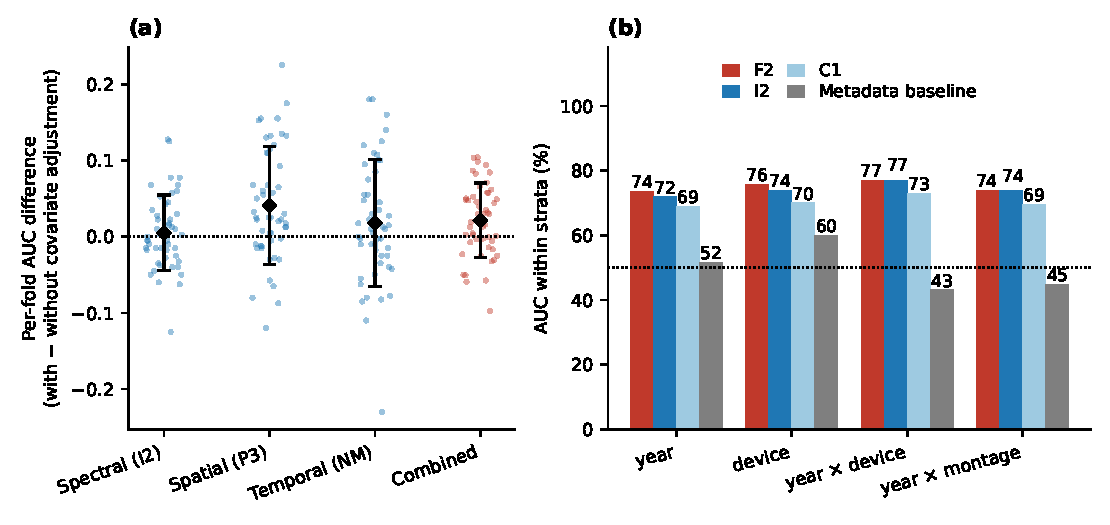
\includegraphics[width=0.80\textwidth]{figures_en/hasil_penyesuaian_strata.pdf}
\caption{(a) Difference in per-fold AUC between models with and without covariate adjustment for the three views and their combined mean (dots: 50 folds; diamond and bar: mean with Nadeau--Bengio corrected 95\% CI; dashed line: zero). (b) AUC of F2, I2, C1, and the acquisition-metadata baseline within strata that compare only patients with and without epilepsy from the same stratum; scores were averaged over 10 repetitions before computing the AUC, which gives higher values than the per-fold AUC (S1.3).}\label{fig:penyesuaian}
\end{figure}

\subsection{Evaluation within strata and age caliper}\label{sec:strata}

To reduce the contribution of acquisition, the comparison was restricted to strata matching year and device (\figref{fig:penyesuaian}b): the acquisition-metadata baseline fell to 43.2, below 50, whereas F2 reached an AUC of 77.0, I2 77.0, and C1 72.9 (AUC of scores averaged over repetitions; the same estimand gives 72.2 for F2 without restriction).
Because the metadata baseline fell below 50, the AUC against 50 is also reported (difference of F2 against it: S2.12).
The difference of F2 against C1 was +4.0 pp (95\% CI $-$1.2 to +9.4; $p = 0.14$), so this signal was not shown to be specific to F2.
Evaluation within strata with an age caliper (\tabref{tab:kaliper}) restricts the comparison to case--control pairs with an age difference $\leq k$ years: 197, 374, and 532 pairs at $k = 5$, 10, and 15, formed by 65--81 of the 100 patients with epilepsy and 76--92 of the 100 without, in 7--9 of the 11 strata that contain both classes (each patient in a median of 2--5 pairs, at most 11--18; S2.15).
The F2 AUC remained 72.6 ($k=5$ years), 73.0 ($k=10$), and 72.0 ($k=15$), with the lower bound of the 95\% CI above 50 ($p_{\mathrm{Holm}} = 0.003$--$0.004$); with equal weight per stratum it was 60.4 (95\% CI 49.7--85.8), 73.6, and 70.8, and without the largest stratum (2012, device X) 73.4--75.5. The demographic baseline fell to about chance and the metadata baseline to 44.2--45.3 (\tabref{tab:kaliper}). At $k=10$, I2 and C1 showed the same signal, and F2 did not differ significantly from C1 (+4.8 pp; $p = 0.33$) or from I2 (+0.3 pp; $p = 0.99$).
Discrimination of the TUEP label therefore persisted among pairs that satisfied these matching restrictions; this does not show that confounding is absent, and the score cannot yet be separated from antiseizure medication and report-derived labels, so it cannot be read as a marker of epilepsy.

\subsection{Equal treatment, selection optimism, and F2-Clean}\label{sec:setara}

With the same treatment for all models, no frozen foundation model exceeded I2, and only BENDR was lower than I2 in the primary family (\tabref{tab:setara43}).
Frozen CBraMod reached a per-fold AUC of 66.2, LaBraM 63.6, and BENDR 53.2 (difference from I2 $-$14.9 pp; Holm 0.03). The 50-feature anatomical compression reached 58.8 (Holm 0.25) and did not raise the AUC.
F2 was the winner in both candidate sets for the optimism correction (pooled AUC 69.4; \tabref{tab:optimisme}).
Conditional on the stored candidates, the selection optimism was 2.0 pp for the 15 main candidates and 3.8 pp for the 50 stored candidates, so the corrected F2 AUC became 67.4 and 65.6; these values are not free of the bias of the whole development process, which the correction does not repeat.
The optimism was larger for 50 candidates than for 15, in line with selection bias growing when more candidates compete on the same patients.
The \textit{studentized max-T} test did not reject that no candidate exceeds the metadata baseline or C1 ($p \geq 0.36$; Holm 0.72 and 1.00). Without the temporal component, F2 (I2 and P3, linear) reached 68.2 (95\% CI 60.0--76.4).
This score could not be distinguished from F2, C1, or the metadata baseline ($p = 0.56$--$0.78$; Holm 1.00; \tabref{tab:s2_p47b}).

\input{\naskahdir/tabel_optimisme}

F2-Clean, which removed age and sex from the final classifier and applied rank-normal before adjustment with a squared age term, reduced the linear dependence of the score on age without a demonstrated change in AUC (\tabref{tab:f2clean}).
The age $r^2$ fell from 0.1322 for F2 ($p<0.001$) to 0.0101 for F2-Clean ($p = 0.39$), which meets the rule, and 0.0027 for F2-Clean without NM ($p = 0.65$); a small $r^2$ with $p>0.10$ does not show that all dependence on age has gone.
NM without age and sex alone did not meet the rule ($r^2$ 0.0211).
The per-fold AUC of F2-Clean was 69.4 (95\% CI 61.8--77.0) and that of F2-Clean without NM 66.8, not significantly different from C1 or the metadata baseline (S2.11).
In the primary family (Holm, four tests), the difference of F2-Clean against F2 was $-$0.3 pp (95\% CI $-$5.6 to +4.9; $p = 0.90$; Holm 1.00).
The difference against C1 was +1.9 pp ($p = 0.64$) and against the metadata baseline +3.9 pp ($p = 0.47$), both with Holm 1.00. The AUC of F2-Clean within year $\times$ device strata with a 10-year age caliper was 77.3 (95\% CI 67.0 to 86.6; $p<0.001$; Holm 0.002), versus 73.0 for F2 on the same pairs. That difference (+4.3 pp; $p = 0.15$; Holm 0.87; \tabref{tab:s2_p45a}) was not significant.
IPW left no detectable linear age dependence in I2 but its AUC was lower (65.3 versus 67.2; table); the 30-window-per-patient sensitivity analysis is in S2.13.

\input{\naskahdir/tabel_f2clean}

Calibration (Brier score 0.221; calibration slope 0.93) and decision curves (S3.6) are descriptive only: the sample prevalence of 50\% and the absence of a defined clinical decision limit their interpretation.
